%----------------------------------------------------------------------------------------
% PACKAGES AND DOCUMENT CONFIGURATIONS
%----------------------------------------------------------------------------------------

  \documentclass[12pt]{article}

  \usepackage{hyperref}
  \usepackage{fancyhdr} % Required for custom headers
  \usepackage{lastpage} % Required to determine the last page for the footer
  \usepackage{extramarks} % Required for headers and footers
  \usepackage[usenames,dvipsnames]{color} % Required for custom colors
  \usepackage{graphicx} % Required to insert images
  \usepackage{listings} % Required for insertion of code
  \usepackage{courier} % Required for the courier font
  \usepackage{lipsum} % Used for inserting dummy 'Lorem ipsum' text into the template
  \usepackage{wrapfig}
  \usepackage{color}
  \usepackage{lscape}

  \setlength\parindent{0pt} % Removes all indentation from paragraphs
  \renewcommand{\labelenumi}{\alph{enumi}.} % Make numbering in the itemize environment by letter rather than number (e.g. section 6)
  \lstset{basicstyle=\ttfamily\footnotesize,breaklines=true}

  % Margins
  \topmargin=-0.4in
  \evensidemargin=0.2in
  \oddsidemargin=-0.2in
  \textwidth=7.0in
  \textheight=9.0in
  % \headsep=0.25in

  % \linespread{1.1} % Line spacing

  \definecolor{dkgreen}{rgb}{0,0.6,0}
  \definecolor{gray}{rgb}{0.5,0.5,0.5}
  \definecolor{mauve}{rgb}{0.58,0,0.82}
  \definecolor{greyish}{rgb}{0.96,0.96,0.96}

  \lstset{
    backgroundcolor=\color{greyish},   % choose the background color; you must add \usepackage{color} or \usepackage{xcolor}
    frame=tblr,
    numbers=left,                       % where to put the line-numbers; possible values are (none, left, right)
    numbersep=5pt,                   % how far the line-numbers are from the code
    numberstyle=\tiny\color{mygray}, % the style that is used for the line-numbers
    language=Ruby,
    aboveskip=3mm,
    belowskip=3mm,
    showstringspaces=false,
    columns=flexible,
    basicstyle={\footnotesize\ttfamily},
    numbers=none,
    numberstyle=\tiny\color{gray},
    keywordstyle=\color{blue},
    commentstyle=\color{dkgreen},
    stringstyle=\color{mauve},
    breaklines=true,
    breakatwhitespace=true
    tabsize=1
  }

  \begin{document}
  \begin{titlepage}

%----------------------------------------------------------------------------------------
% TITLE PAGE INFORMATION
%----------------------------------------------------------------------------------------
 \newcommand{\HRule}{\rule{\linewidth}{0.5mm}} % Defines a new command for the horizontal lines, change thickness here
  \begin{center} % Center everything on the page

  %----------------------------------------------------------------------------------------
  % HEADING SECTIONS
  %----------------------------------------------------------------------------------------
  \textsc{\large Faculty of Computers, Informatics and Microelectronics}\\[0.5cm]
  \textsc{\large Technical University of Moldova}\\[1.2cm] % Name of your university/college
  \vspace{35 mm}
  \textsc{\Large PAD}\\[0.5cm] % Major heading such as course name
  %\textsc{\large Laboratory work \#1-3}\\[0.5cm] % Minor heading such as course title
  \textsc{\large Laboratory work \# 6}\\[0.5cm] % Minor heading such as course title

  %----------------------------------------------------------------------------------------
  % TITLE SECTION
  %----------------------------------------------------------------------------------------
  \vspace{10 mm}
  \HRule \\[0.4cm]
  { \large \bfseries  Building a Proxy with Shared Databases.}\\[0.4cm] % Title of your document
  \HRule \\[1.5cm]

  %----------------------------------------------------------------------------------------
  % AUTHOR SECTION
  %----------------------------------------------------------------------------------------
      \vspace{25mm}

      \begin{minipage}{0.4\textwidth}
      \begin{flushleft} \large
      \emph{Authors:}\\
      \textbf{Petru \textsc{Negrei}} \\
      Victor \textsc{Vasilica}
      \end{flushleft}
      \end{minipage}
      ~
      \begin{minipage}{0.4\textwidth}
      \begin{flushright} \large
      \emph{Supervisor:} \\
      D. \textsc{Ciorba} % Supervisor's Name
      \end{flushright}
      \end{minipage}\\[4cm]

      \vspace{5 mm}
      % If you don't want a supervisor, uncomment the two lines below and remove the section above
      %\Large \emph{Author:}\\
      %John \textsc{Smith}\\[3cm] % Your name

      %----------------------------------------------------------------------------------------
      % DATE SECTION
      %----------------------------------------------------------------------------------------

      {\large December 2014}\\[3cm] % Date, change the \today to a set date if you want to be precise

      %----------------------------------------------------------------------------------------
      % LOGO SECTION
      %----------------------------------------------------------------------------------------

      %\includegraphics{Logo}\\[1cm] % Include a department/university logo - this will require the graphicx package

      %----------------------------------------------------------------------------------------

      \vfill % Fill the rest of the page with whitespace
      \end{center}
      \end{titlepage}

      % \newpage
      % \tableofcontents
      % \newpage

%----------------------------------------------------------------------------------------
% Introduction
%----------------------------------------------------------------------------------------

  \section{Introduction}

  \subsection{Topic}

   Build a Proxy that will link the client with the main server and assure the integrity 
   of data among servers.

  \subsection{Generic requirements}

  \subsubsection{Task}

  Develop a system of distributed heterogeneous data, centralized in one node type warehousing.

  \subsubsection{Report}

  Report will contain a short description of work done, and will present necesary information
  about tools, algorithms used or studied.

%----------------------------------------------------------------------------------------
% Implementation
%----------------------------------------------------------------------------------------
  
  \section{Structure}

    \begin{minipage}[b]{1.0\linewidth}
      \begin{center}
        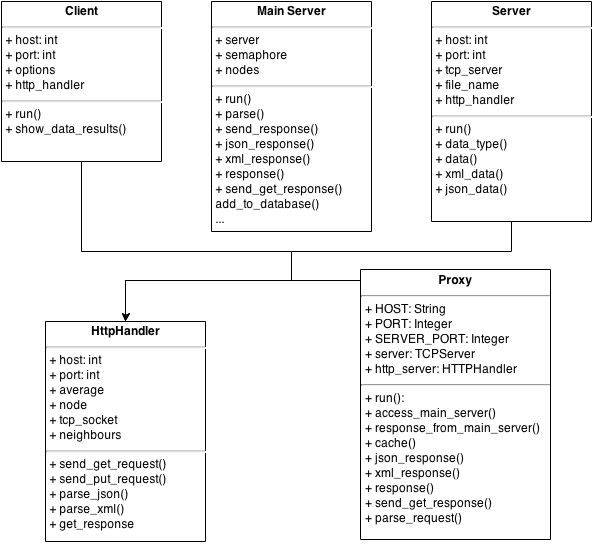
\includegraphics[width=0.65\textwidth]{diagram}
         \\ Fig. 1 Class diagram
      \end{center}
    \end{minipage}
    
    \vspace{0.5cm}

    Above you can see the structure of the application, (the structure remained the same) there are 
    represented the classes used  and their variables and methods.
    The application is composed of three main clasess \textit{Client}
    and \textit{Server} and \textit{Main Server}, and now also the \textit{Proxy} class. \\

    The \textit{Client}, \textit{Server}, \textit{Proxy} classes use the \textit{HttpHandler} helper class in order to
    send the necesary requests to the \textit{Main Server} and also recieve the response from it. \\ 

    The requests are handled and analyzed on \textit{Main Server} in different threads and saved on 
    a single database, the database doesn't duplicate request, if it receives a data that already that is in
    database it will update the fields of it. 


  \section{Implementation}

    \subsection{Proxy}

    Here I will explain the structure of the \textit{Proxy} class. The description for 
    other class in the system you can find in the previous laboratory work. 

    The most important function of the \textit{Proxy} is to receive \textit{GET} request
    from client, and to pass this requests to the server part. Then it receives the 
    response from main server and sends it back to the client. At this level it is also 
    implemented caching of the request, which was implemented toghether with Victor.

    The \textit{run} function is the function that receives requests from client in a thread safe way 
    and depending if the requsts was already in the cache to send the cached response or to 
    access main server and cached and send response from it to the client.

    \begin{lstlisting}
    # ...
     def run
        loop do
         Thread.start(server.accept) do |client|
            http_header = client.gets("\r\n\r\n")

            unless redis.exists(http_header)
              @http_server = HttpHandler.new HOST, SERVER_PORT
              access_main_server(http_header)
            end

            send_get_response(client, redis.get(http_header))
            client.close
          end
        end
      end
    # ... 
    \end{lstlisting}

    Below I will describe each function utility. 

    \begin{itemize}
      \renewcommand{\labelitemi}{$\circ$}
      \item \textit{initialize} - create a TCPServer to listen to the clients request, and also \textit{Redis} object
      to store the cache of the requests.
      \item \textit{access\_main\_server} - to send request to the main server and call the \textit{cache} method.
      \item \textit{response\_from\_main\_server} - contains the response from server in different formats.
      \item \textit{cache} - save the cache key and value with a given interval of time.
      \item \textit{json\_response} - returns the json response. 
      \item \textit{xml\_response} - returns the xml response.
      \item \textit{response} - the method that returns the data depending of the user request.
      \item \textit{send\_get\_response} -  sends the response in the right format with the right data.
      \item \textit{parse\_request} - return the type and url from the client request.
    \end{itemize}

    \begin{lstlisting}
     # ... 
      class Proxy
        HOST = 'localhost'
        PORT = 8001
        SERVER_PORT = 8000

        attr_reader :server, :http_server, :redis

        def initialize
          @server = TCPServer.new HOST, PORT
          @redis = Redis.new
          @redis.flushall
        end

     # ... 

      def access_main_server http_header
        puts "new data"
        resp = response_from_main_server(http_header)
        cache(http_header, resp, 60)
        resp
      end

      def response_from_main_server http_header
        url, _, type = parse_request(http_header)
        http_server.send_get_request("/" << url, type)
        (type == 'json') ? json_response : xml_response
      end

      def cache key, value, expires_at
        redis.set(key, value)
        redis.expire(key, expires_at)
      end

     # ... 
    \end{lstlisting}

    \subsection{Server Side}

    The server part was done by Vasilica Victor and the caching functionality was implemented together.

    \section{Conclusion}

    After implementing this laboratory work, I learn how to build a Proxy that will allow client to communicate
    with different main Servers, and to receive response from them. I implemented a caching system
    that will optimize the requests received and send the response faster without accessing the server.

    \textbf{Link to Repository: } \url{https://gitlab.ati.utm.md/petru.negrei/lab6}

   \section{References}

   \begin{itemize}
      \item Redis \url{http://redis.io/}
      \item Ruby Socket \url{http://www.ruby-doc.org/stdlib-1.9.3/libdoc/socket/rdoc/Socket.html}
      \item Ruby TCP  Socket \url{http://www.ruby-doc.org/stdlib-1.9.3/libdoc/socket/rdoc/TCPSocket.html}
      \item Ruby Mutex \url{http://wwwi.ruby-doc.org/core-2.1.4/Mutex.html}
      \item Ruby JSON \url{http://www.ruby-doc.org/stdlib-2.0.0/libdoc/json/rdoc/JSON.html}
      \item Ruby OptionParser \url{http://ruby-doc.org/stdlib-2.1.0/libdoc/optparse/rdoc/OptionParser.html}
   \end{itemize}

\end{document}